\Section{StreamIt Programming Language}
\label{sec:streamit}

StreamIt  is   an  architecture independent language that is
designed for  stream programming. In StreamIt, programs are
represented as graphs where  nodes represent  computation and edges
represent FIFO-ordered communication of data over tapes.
The language features several novelties that are essential
for large scale program development: the language is modular,
parameterizable, malleable and architecture independent. In addition,
the language exposes the widespread parallelism and communication
patterns that are inherent in many streaming programs.

\SubSection{Filters as Programmable Units}
In  StreamIt, the  basic programmable  unit is a {\it filter}.   Each
filter contains  a work  function that executes atomically,  popping
(i.e., reading)  a fixed number  of items  from the  filter input tape
and pushing (i.e., writing) a fixed number of items to the filter
output tape.  A filter  may also {\tt peek} at a given index on its
input tape without  consuming  the  item;  this makes  it simple  to
represent computation over a sliding window or performing permutations
on the input stream.   The {\tt push}, {\tt pop}, and {\tt peek} rates
are declared as part of  the work  function,  thereby enabling  the
compiler  to apply various optimizations and construct efficient
execution schedules. 

A filter is akin to a class in object oriented programming with the
work function serving as the main method. A filter is parameterizable,
and this allows for greater malleability and code reuse.  An example
filter is shown in Figure~\ref{fig:zigzag-filter}. It implements the
zig-zag scanning pattern used in the run-length processing of
quantized DCT coefficients in MPEG. The zig-zag scan pattern is
illustrated in Figure~\ref{fig:zigzag}. Typically, the zig-zag scan
operates on a 8x8 matrix. An instantiation of a filter can specify the
matrix dimmensions, as well as the desired ordering. In MPEG, there
are two possible scan orders. The {\tt Order} array can define the
specific order. For example, to implement the order shown in
Figure~\ref{fig:zigzag}(a), the {\tt Order} array is defined as shown
in Figure~\ref{fig:zigzag-order}.

\begin{figure}[t]
\begin{center}
\vspace{-12pt}
% \framebox{
% \includegraphics[scale=1, angle=0]{./zigzag.eps}
%}
% \vspace{-6pt}
% \nocaptionrule
 \caption{Zig-Zag scan patterns allowed by MPEG.}
 \label{fig:zigzag}
%\vspace{-18pt}
\end{center}
\end{figure}

\begin{figure}[t]
\begin{scriptsize}
% {\small
\begin{verbatim}
int->int filter ZigZagScan(int N, int[N] Order)
{
  work pop N push N {
    for (int i = 0; i < N; i++) {
      int pixel = peek(Order[i]);
      push(pixel);
    }
    for (int i = 0; i < N; i++) {
      pop();
    }
  }
}
\end{verbatim}
% }
\end{scriptsize}
\vspace{-3pt}
\caption{Example filter implementing zig-zag scanning.}
\label{fig:zigzag-filter}
\end{figure}

\begin{figure}[t]
\begin{scriptsize}
% {\small
\begin{verbatim}
int[64] Ordering = 
  {00, 01, 05, 06, 14, 15, 27, 28,
   02, 04, 07, 13, 16, 26, 29, 42,
   03, 08, 12, 17, 25, 30, 41, 43,
   09, 11, 18, 24, 31, 40, 44, 53,
   10, 19, 23, 32, 39, 45, 52, 54,
   20, 22, 33, 38, 46, 51, 55, 60,
   21, 34, 37, 47, 50, 56, 59, 61,
   35, 36, 48, 49, 57, 58, 62, 63};
\end{verbatim}
% }
\end{scriptsize}
\vspace{-3pt}
\caption{Example zig-zag order specification for filter.}
\label{fig:zigzag-order}
\end{figure}

\SubSection{Hierarchical Streams}

{\bf update to reflect top level streamit pipeling for decoder}

In StreamIt, the
application developer focuses on the hierarchical assembly of the
stream graph and its communication topology, rather than on the 
explicit management of the data buffers between filters.
StreamIt provides three hierarchical structures for composing filters
into larger stream graphs (see Figure~\ref{fig:containers}). The 
{\it pipeline} construct composes streams in sequence, with the output
of one connected to the input of the next.   An example of a pipeline
appears in Figure~\ref{fig:pipeline}.

{\bf update to reflect parallelization of motion compation across
  luminance and chrominance channels}

The {\it splitjoin} construct distributes data to a set of parallel
streams, which are then joined together in a roundrobin fashion.  In
a splitjoin, the {\it splitter} performs the data scattering, and the
{\it joiner} performs the gathering. A splitter is a specialized
filter with a single input and  multiple output channels. On 
every execution step, it can distribute its output to any one of
its children in either a {\it duplicate} or a {\it roundrobin}
manner. For the former, incoming data are replicated to every
sibling connected to the splitter. For the latter, data are scattered
in a roundrobin manner, with each item sent to exactly one child
stream, in order.  The splitter type and the weights for distributing data to
child streams are declared as part of the syntax (e.g., \texttt{split
duplicate} or \texttt{split roundrobin($w_1,\ldots,w_n$)}). The
splitter counterpart is the joiner. It is a specialized filter with  
multiple input channels but only one output channel. The joiner
gathers data from its predecessors in a roundrobin manner (declared
as part of the syntax) to produce a single output stream.

StreamIt also provides a {\it feedback loop} construct for introducing
cycles in the graph. This stream construct is not used in the decoder,
but can occur in the MPEG encoder.

%% XXX update figures using MPEG pipeline and splitjoin

\begin{figure}[t]
\begin{center}
%\vspace{-24pt}
% \framebox{
 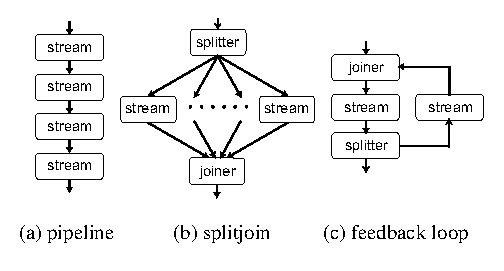
\includegraphics[scale=1, angle=0]{./constructs-eg.eps}
%}
% \vspace{-6pt}
% \nocaptionrule
 \caption{Hierarchical streams in StreamIt.}
 \label{fig:containers}
\end{center}
\end{figure}

\begin{figure}[t]
\begin{center}
\vspace{-12pt}
% \framebox{
% 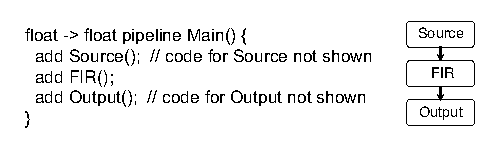
\includegraphics[scale=1, angle=0]{./pipeline-eg.eps}
%}
% \vspace{-6pt}
% \nocaptionrule
 \caption{Example deconding pipeline.}
 \label{fig:pipeline}
%\vspace{-18pt}
\end{center}
\end{figure}

{\bf need to introduce messaging and talk about it}